\section{Controlling}

To control the speed of the DC motor a controller will have to be implemented in to the system. A block diagram of the DC motor in figure~\ref{fig:dcmotormodel} is shown in figure~\ref{fig:dcblock}. From the block diagram a transfer function $P(s)$ for the motor can be derived as P(s) as seen in equation~\ref{eq:fullplant} on the form in equation~\ref{eq:simpleplant} .

\begin{figure}[!h]
	\centering
	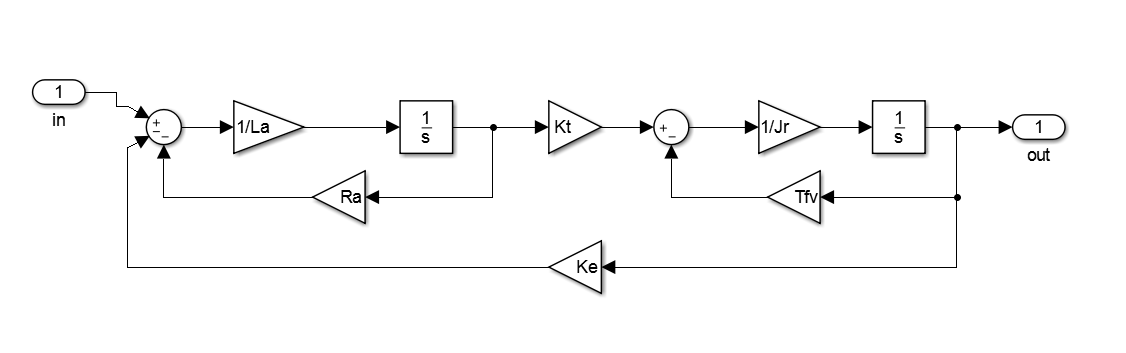
\includegraphics[width=.75\linewidth]{graphics/dcblockdiagram}
	\caption{A block diagram of the Dc motor}
	\label{fig:dcblock}
\end{figure}


\begin{equation}
\label{eq:fullplant}
P(s) = \dfrac{\dfrac{K_m}{J_r L_a}}{s^2 + \dfrac{J_r R_a + L_a Tfv}{J_r L_a}s + \dfrac{R_a Tfv +K_m^2}{J_r L_a}}
\end{equation}

\begin{equation}
\label{eq:simpleplant}
P(0) \dfrac{b_0}{s^2 a_1 s + a_0}
\end{equation}


The controller will be placed before the input of the motor monitoring the output through a feedback. the system is shown in~\ref{fig:controlsystem} where the plant is the DC motor. The transfer function $H(s)$ is shown in equation~\ref{eq:tfsystem} where $C(s)$ is the transfer function of the controller
 
\begin{figure}[!h]
	\centering
	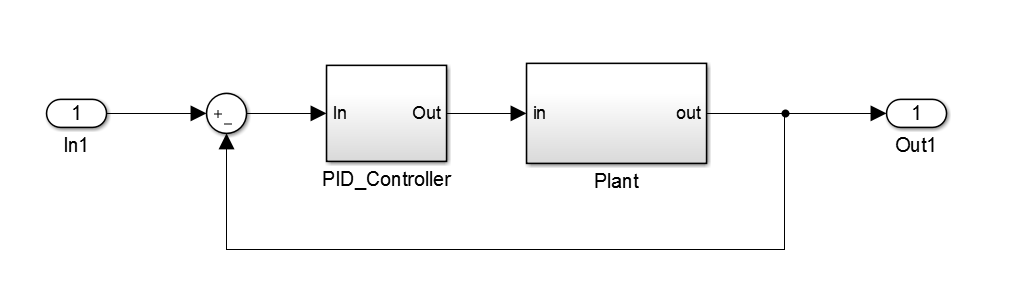
\includegraphics[width=.75\linewidth]{graphics/controlsystem}
	\caption{Block diagram of the control system}
	\label{fig:controlsystem}
	
\end{figure}

\begin{equation}
\label{eq:tfsystem}
H(s) = \dfrac{C(s)P(s)}{1+C(s)P(s)}
\end{equation}


\subsection{PID - controller}
 A commonly used controller is the PID-controller\cite{feedback}. The name comes from its three adjustable parameters, the proportional gain $K_{P}$, integral gain $K_{I}$ and the derivative gain $K_{D}$. Reason for its popularity is the wide range of operating conditions as well being relatively easy to understand.
 A block diagram for the PID-controller can be seen in figure~\ref{fig:pidblock} and equation~\ref{eq:pid} shows the transfer function of the PID-controller.  

\begin{figure}[!h]
	\centering
	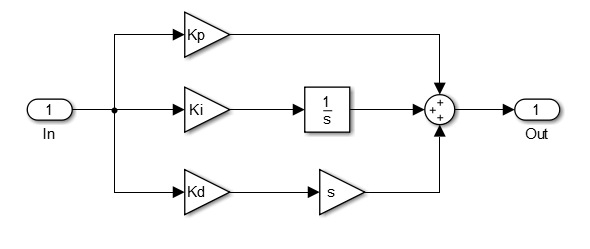
\includegraphics[width=.7\linewidth]{graphics/pidcontroller}
	\caption{Block diagram of the PID-controller}
	\label{fig:pidblock}
\end{figure}

\begin{equation}
\label{eq:pid}
K_P + \dfrac{K_I}{s} +K_D s
\end{equation}

\subsection{Noise Filtering}

The derivative part of the PID-controller will try to reduce every sudden change in the system. This is what helps the system stop oscillating. However when noise is introduces to the system, the derivative term acts on the fast, sudden change and can destabilize the system. In other words the derivative term can and will increase the noise. For this reasons a low pass filter is needed on the derivative path. This is done with changing $s$ on the derivative gain to $N/(s + N)$ where $N$ is $1/T_f$ and $T_f$ is the filter time constant and N is the cut off frequency. The block diagram for the controller then becomes as seen in figure~\ref{fig:pidfilter} having the transfer function $C(s)$ seen in equation~\ref{eq:pidfilter}.

\begin{figure}[!h]
	\centering
	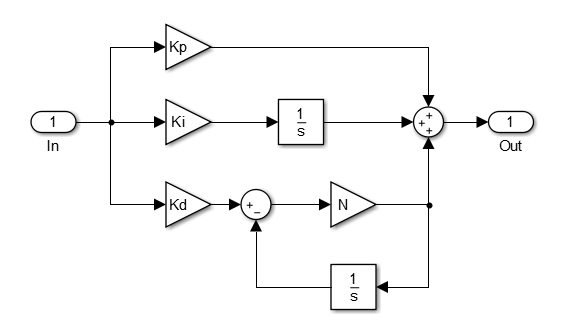
\includegraphics[width=.7\linewidth]{graphics/pidwfilter}
	\caption{Block diagram of the PID-controller with an added filter}
	\label{fig:pidfilter}
\end{figure}

\begin{equation}
\label{eq:pidfilter}
K_P + \dfrac{K_I}{s} + \dfrac{N K_D s}{s + N}
\end{equation}

\subsection{Anti-Windup Design}

\subsection{Controller Gain Design}

\begin{equation}
\centering
\label{eq:settling}
\alpha = \dfrac{1.5(1 + n)}{T_s}
\end{equation}

\begin{equation}
\centering
\label{eq:standard}
s^n + d_{n-1}s^{n-1} + \cdots + d_1 s + d_0 
\end{equation}


\begin{table}[!h]
	\caption{ Coefficients of
		closed loop differential
		equation based on settling
		time formula\cite{feedback}}
	\centering
	\begin{tabular}{|c|c|c|c|}
		\hline
		n & 2 & 3 & 4\\
		\hline
		$d_0$ & $\alpha^2$ & $\alpha^3$ & $\alpha^4$\\ 
		$d_1$ & $2\alpha$ & $3\alpha^2$ & $4\alpha^3$\\
		$d_2$ & - & $3\alpha$ & $6\alpha^2$\\
		$d_0$ & - & - & $4\alpha$\\
		\hline
		

	\end{tabular}
\end{table}
